\documentclass{article}
\usepackage[margin=1.1in]{geometry}
\usepackage{graphicx}
\usepackage{amsmath}
\usepackage{amssymb}
\usepackage{hyperref}
\usepackage{booktabs}
\usepackage{xcolor}
\usepackage{listings}
\usepackage{tcolorbox}
\usepackage{pdfpages}
\tcbuselibrary{listings, skins, breakable}

% Output box environment (black background, white text)
\newtcolorbox{outputbox}[1]{
    arc=3mm,
    boxrule=1pt,
    colback=black!85!white,
    colframe=black,
    coltext=white,
    title={\textbf{#1}},
    fontupper=\ttfamily\scriptsize,
    left=2mm, right=2mm, top=2mm, bottom=2mm,
    fontupper=\ttfamily\scriptsize\obeylines,
    breakable
}

% Python code box environment
\lstdefinestyle{pythonstyle}{
    language=Python,
    basicstyle=\ttfamily\scriptsize,
    keywordstyle=\color{blue!80!black}\bfseries,
    stringstyle=\color{green!60!black},
    commentstyle=\color{gray}\itshape,
    showstringspaces=false,
    numbers=left,
    numberstyle=\tiny\color{gray},
    numbersep=3.5pt,
    breaklines=true,
    tabsize=4
}
\newtcblisting{pythonbox}[1]{
    arc=3mm,
    boxrule=1pt,
    colback=yellow!5!white,
    colframe=yellow!50!black,
    title={\textbf{#1}},
    listing only,
    listing style=pythonstyle,
    breakable
}

% ── Title ─────────────────────────────────────────────────────────────────────
\begin{document}

\begin{titlepage}
\begin{center}


\includegraphics[width=0.55\textwidth]{images/ozu.png}\\[2cm]

\rule{\linewidth}{0.5mm}\\[0.4cm]

{ \LARGE
  \textbf{PHYS551: Advanced Monte Carlo Methods}\\[0.4cm]
  \emph{Homework 6}\\[0.4cm]
}
\rule{\linewidth}{0.5mm}\\[0.4cm]

\hfill\hfill

\linewidth=0.8\textwidth
\begin{minipage}{0.4\textwidth}
    \begin{flushleft} \large
        \emph{Student:}\\
        Ömer Faruk \textsc{Avcı}
    \end{flushleft}
\end{minipage}
~
\begin{minipage}{0.5\textwidth}
    \begin{flushright} \large
        \emph{Instructor:}\\
        Prof. Dr. Taylan \textsc{Akdo\u{g}an}\\[0.1cm]
    \end{flushright}
\end{minipage}

\vfill

\textsc{\large Department of Electrical and Electronics Engineering}\\[0.4cm]

{\large \today}

\end{center}
\end{titlepage}

\section*{Disclosures and References}

\textbf{AI Usage Disclosure:} In accordance with the course policy, I would like to declare the extent of AI assistance used in this assignment:

\begin{itemize}
    \item \textbf{Code \& Visualizations:} AI tools were utilized to assist in debugging PyMC model definitions and to refine the output plots.
    \item \textbf{Document Preparation:} AI assistance was used to construct and format the LaTeX document.
\end{itemize}

\newpage

% =============================================================
% PROBLEM 1
% =============================================================
\section*{Problem 1: Model 1 -- Basquin's Equation}

\subsection*{Part (a): Prior Predictive Check}

Basquin's equation in log-space is:
\[
\ln(N_i) = \alpha - \beta \ln(S_i), \quad N_i \sim \text{LogNormal}(\mu_i,\, \sigma)
\]

I centered the log-stress by subtracting $\overline{\ln S}$ to reduce correlation between $\alpha$ and $\beta$ during sampling. The priors I used:
\begin{itemize}
    \item $\alpha \sim \mathcal{N}(13.5,\; 5)$ -- around expected log-life at mean stress
    \item $\beta \sim \mathcal{N}(10,\; 5)$ -- positive so that life decreases with stress
    \item $\sigma \sim \text{HalfNormal}(1)$
\end{itemize}

I sampled 500 prior predictive curves and plotted them on a log-log scale. Out of 500 draws, only 10 had $\beta < 0$ (about 2\%), so the priors are reasonable.

\begin{figure}[h!]
    \centering
    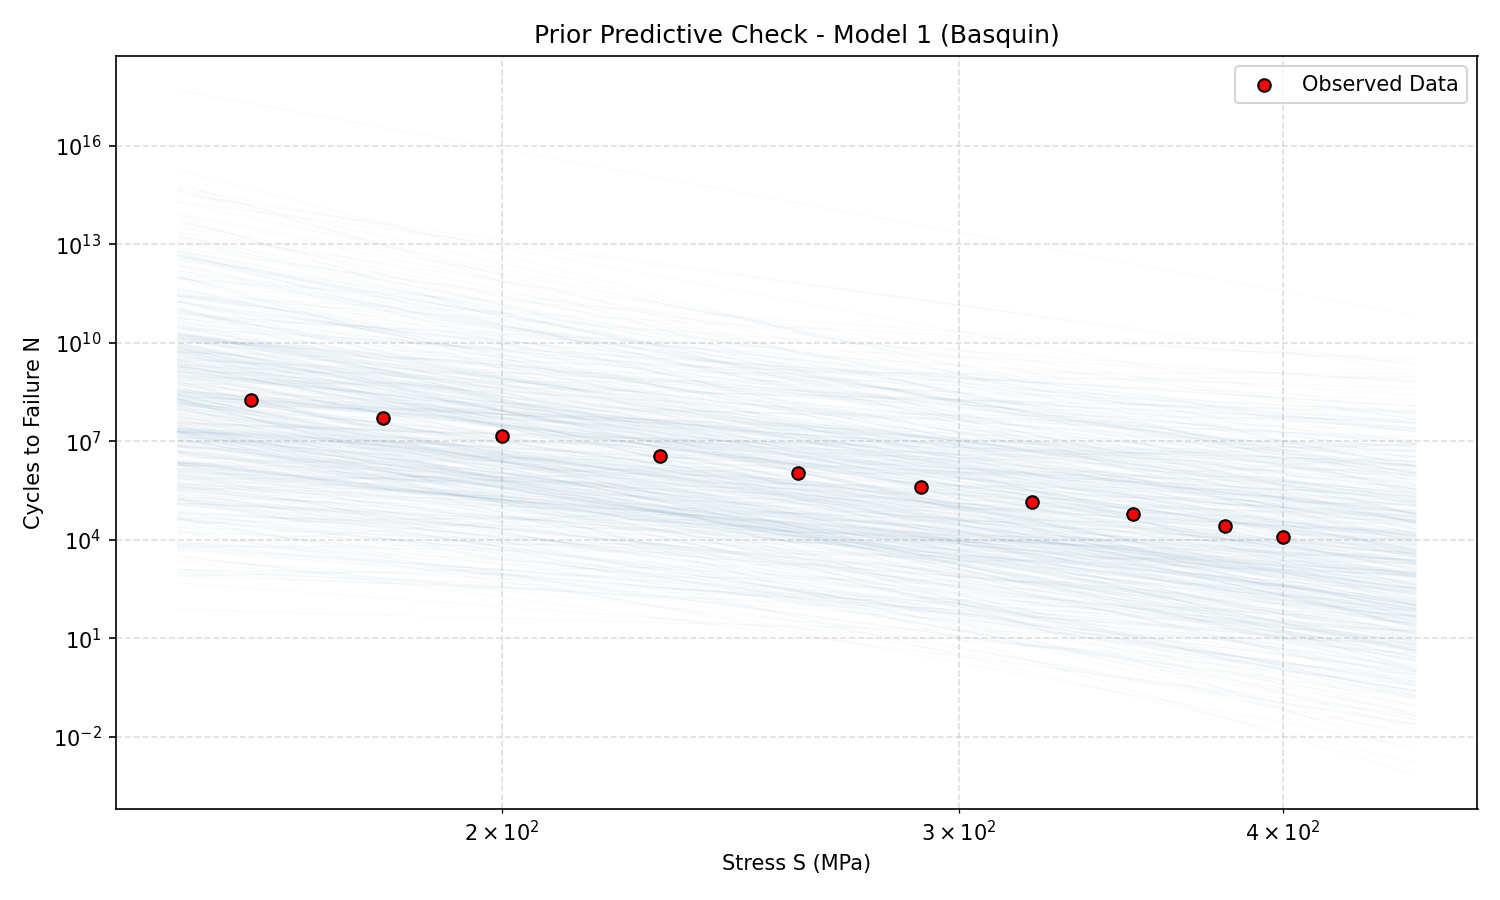
\includegraphics[width=0.85\textwidth]{images/prior_predictive_m1.png}
    \caption{Prior predictive S-N curves (500 draws). Data shown in red.}
\end{figure}

\newpage
\subsection*{Part (b): Inference \& Diagnostics}

Ran NUTS with 4 chains, 1000 tuning, 2000 draws each. Set \texttt{target\_accept = 0.95}.

\begin{outputbox}{Model 1 -- MCMC Summary}
Parameter    Mean      SD      R-hat    Bulk ESS    Tail ESS
---------------------------------------------------------
alpha       13.765   0.044     1.00      5161        4544
beta        10.224   0.142     1.00      5564        4150
sigma        0.134   0.042     1.00      4221        4235

Divergent transitions: 0
\end{outputbox}

$\hat{R} = 1.00$ across the board, ESS values are all well above 400, and no divergences. The trace plots show good mixing across all 4 chains.

\begin{figure}[h!]
    \centering
    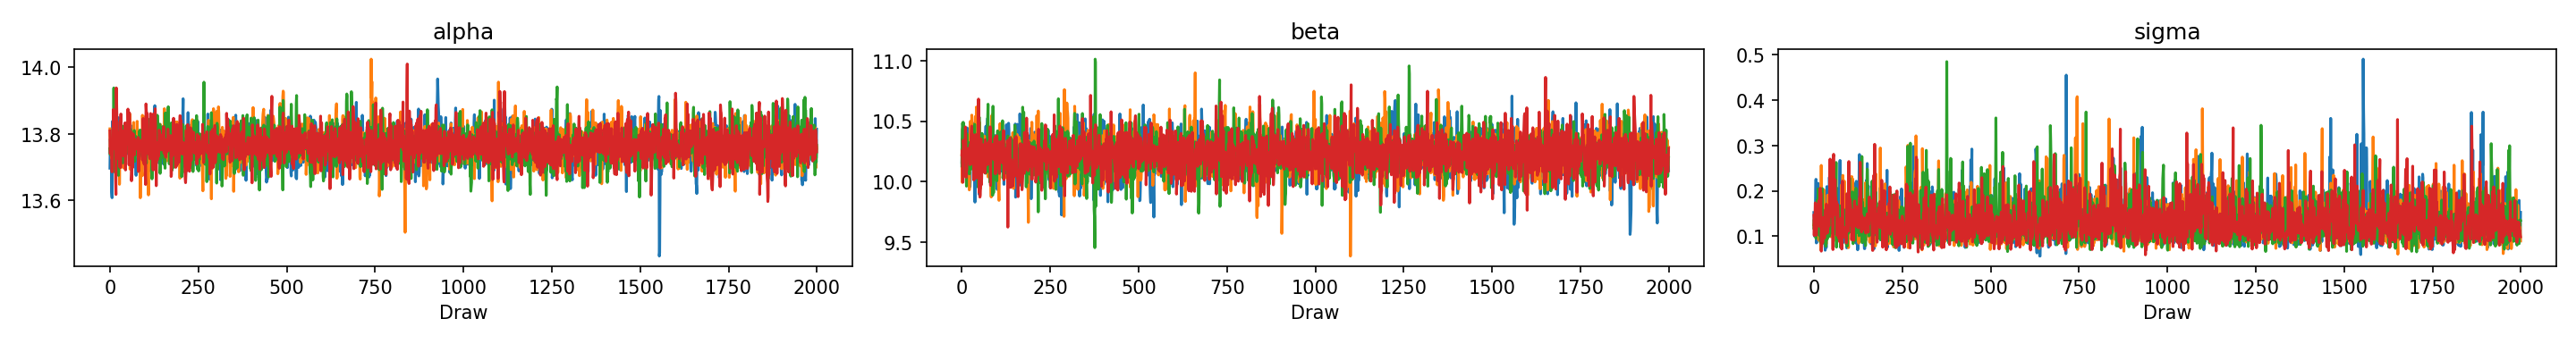
\includegraphics[width=\textwidth]{images/trace_m1.png}
    \caption{Trace plots for Model 1. All chains overlap well.}
\end{figure}

\subsection*{Part (c): Posterior Predictive Check}

Generated the posterior predictive distribution by propagating the posterior samples through the model (including the $\sigma$ noise). Computed the 95\% credible interval from the 2.5th and 97.5th percentiles.

\begin{figure}[h!]
    \centering
    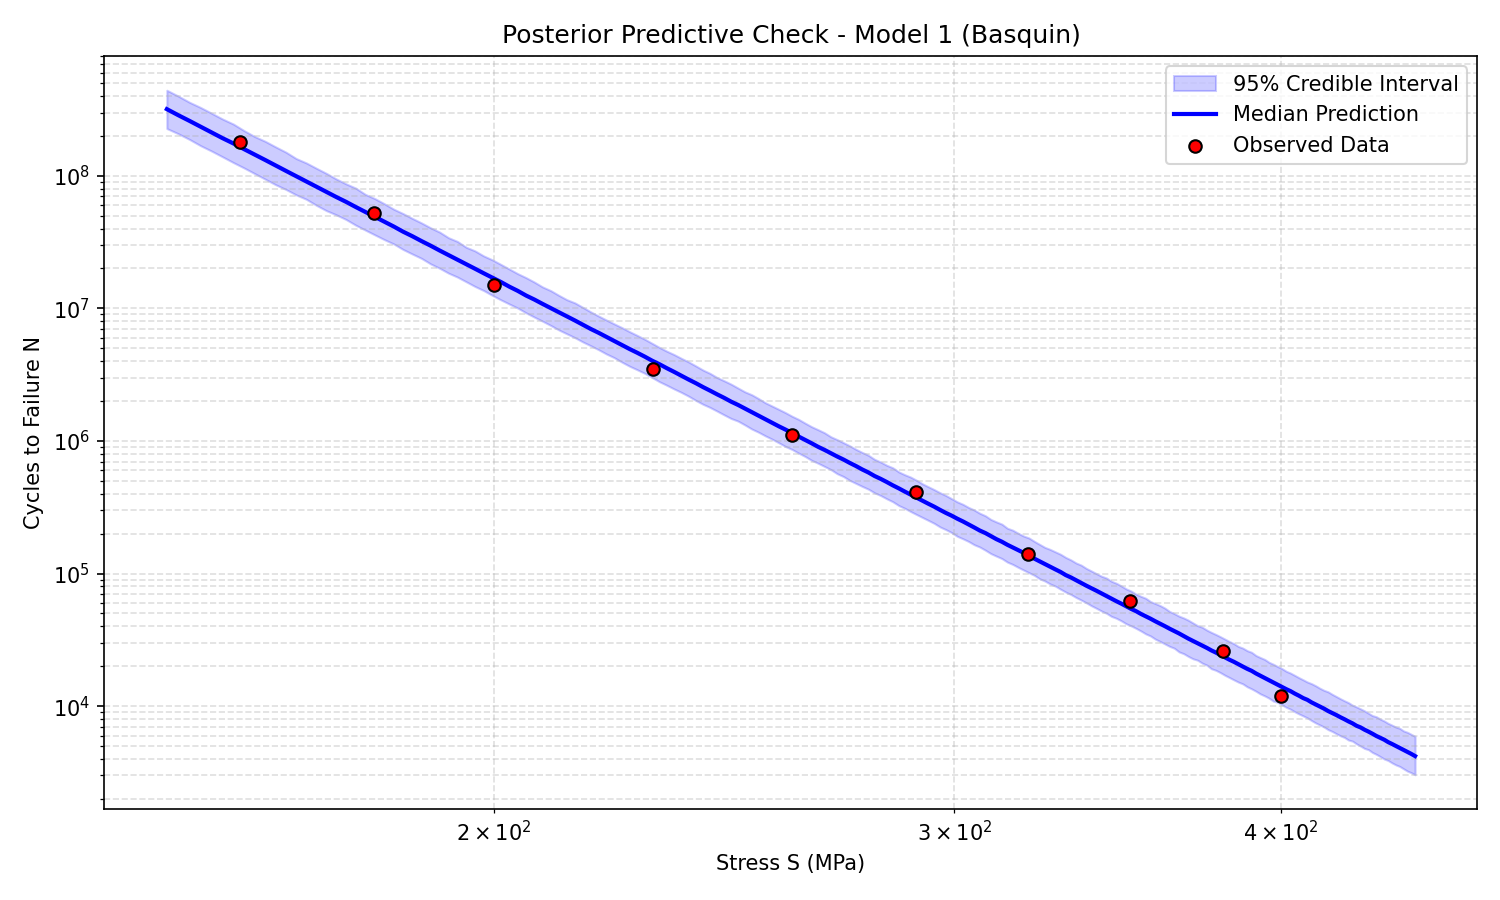
\includegraphics[width=0.85\textwidth]{images/ppc_m1.png}
    \caption{Posterior predictive check. All data points fall inside the 95\% band.}
\end{figure}

All 10 data points sit comfortably within the credible band and the median line tracks them closely. The band is fairly narrow ($\sigma \approx 0.13$), which tells us Basquin's power law is a pretty good fit for this data.

\newpage

% =============================================================
% PROBLEM 2
% =============================================================
\section*{Problem 2: Model 2 -- Stromeyer's Equation}

\subsection*{Part (a) \& (b): Model and Inference}

Stromeyer adds a fatigue limit $S_e$:
\[
\mu_i = \alpha - \beta \ln(S_i - S_e)
\]
I used $S_e \sim \text{Uniform}(0, 155)$ so that $S_i - S_e > 0$ for all data points (lowest stress is 160 MPa). The priors for $\alpha$ and $\beta$ are similar to Model 1, though I widened $\alpha$ to $\mathcal{N}(40, 15)$ since the Stromeyer parameterization shifts the intercept higher.

This model has a tricky posterior geometry -- when $S_e$ gets close to the lowest stress value, tiny changes in $S_e$ cause huge swings in $\ln(S - S_e)$, creating a funnel shape. To deal with this I set \texttt{target\_accept = 0.99} and doubled the tuning steps to 2000. All 4 chains hit the maximum tree depth warning, which is expected for this kind of geometry, but the sampler still converged with 0 divergences.

\begin{outputbox}{Model 2 -- MCMC Summary}
Parameter    Mean      SD      R-hat    Bulk ESS    Tail ESS
---------------------------------------------------------
alpha        62.7     4.6      1.00       977        1390
beta          8.96    0.72     1.00       982        1411
sigma         0.144   0.052    1.00      1619        1741
Se           30.0    16.7      1.00       979        1217

Divergent transitions: 0
\end{outputbox}

The ESS values are noticeably lower than Model 1 (around 1000 vs 5000), which reflects the harder posterior geometry. Still above the minimum threshold though.

\begin{figure}[h!]
    \centering
    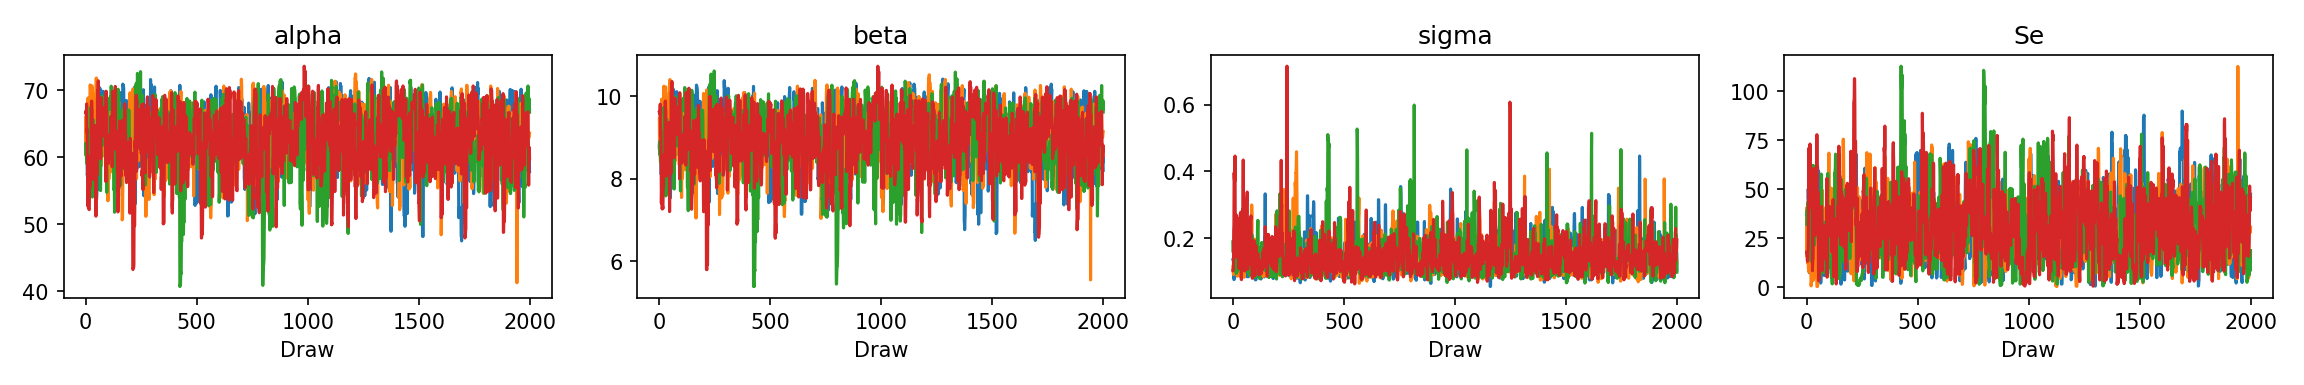
\includegraphics[width=\textwidth]{images/trace_m2.png}
    \caption{Trace plots for Model 2. $S_e$ explores a wide range but chains still mix.}
\end{figure}

\subsection*{Part (c): Fatigue Limit Results}

\begin{outputbox}{Fatigue Limit Estimate}
Se (Fatigue Limit):
  Mean = 30.0 MPa
  94% HDI = [0.6, 58.1] MPa
\end{outputbox}

The estimated fatigue limit is $S_e = 30.0 \pm 16.7$ MPa. The 94\% HDI is very wide and almost touches zero, meaning the data doesn't really constrain $S_e$ well. This makes sense physically -- our tested stresses (160--400 MPa) are all way above any reasonable endurance limit for this alloy, so the data just doesn't have enough information to pin down where the material would stop failing.

\newpage

% =============================================================
% PROBLEM 3
% =============================================================
\section*{Problem 3: Model Comparison (PSIS-LOO)}

\subsection*{Part (a): LOO Cross-Validation}

I used \texttt{az.compare()} to run PSIS-LOO on both models.

\begin{outputbox}{LOO Comparison}
             rank    ELPD    p\_eff   ELPD\_diff   weight    SE     dSE   warning
-------------------------------------------------------------------------------
Basquin        0    -130.0   2.2       0.0        1.0      9.6    0.0   False
Stromeyer      1    -130.0   3.6      -2.0        0.0      8.9    2.1   True
\end{outputbox}

One thing worth noting: the Stromeyer model triggered a Pareto $\hat{k} > 0.7$ warning during LOO computation, which means that for at least one data point, the importance sampling approximation is unreliable. This happens when removing a single observation changes the posterior significantly -- basically one of the data points is very influential for the Stromeyer model. The Basquin model had no such issue.

\begin{figure}[h!]
    \centering
    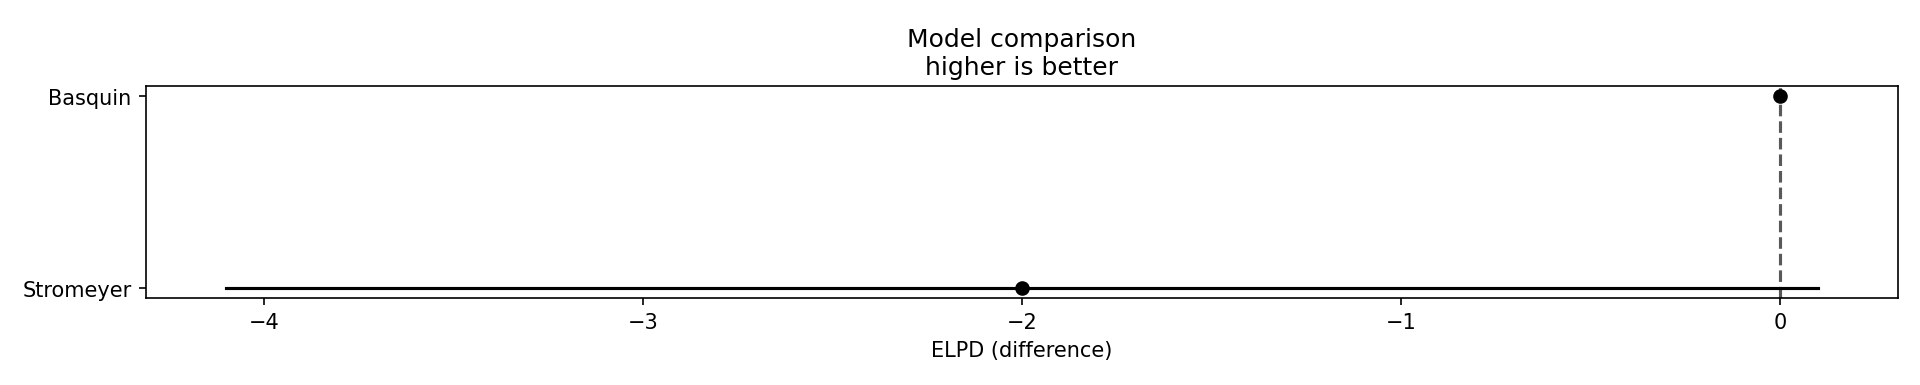
\includegraphics[width=0.85\textwidth]{images/loo_comparison.png}
    \caption{ELPD comparison. Higher is better. Error bars show standard error.}
\end{figure}

\subsection*{Part (b): Conclusion}

The ELPD difference between the two models is $\Delta\text{ELPD} = 2.0$ with a standard error of $2.1$. Since the difference is smaller than the standard error, neither model is clearly better at predicting unseen data. However, there are several reasons to prefer the simpler Basquin model:

First, Basquin uses fewer effective parameters ($p_{\text{eff}} = 2.2$ vs $3.6$) and Occam's razor favors parsimony when predictive power is equivalent. Second, the Stromeyer model triggers the Pareto $\hat{k}$ diagnostic warning, indicating its LOO estimate is less trustworthy. Third, the fatigue limit $S_e$ has such a wide posterior (HDI nearly touching zero) that the data doesn't support the existence of an endurance limit in this stress range. The added complexity of Stromeyer's equation is not justified here, and Basquin's power law remains the better engineering model for this dataset.

\newpage

% =============================================================
% APPENDIX
% =============================================================
\section*{Appendix: Source Code}

\begin{pythonbox}{hw6.py -- Complete Implementation}
"""
# PHYS 551: Advanced Monte Carlo Methods
# Homework 6 - Source Code
# Student: Omer Faruk Avci
# Instructor: Prof. Dr. Taylan Akdogan
"""
import pymc as pm
import numpy as np
import matplotlib.pyplot as plt
import arviz as az

# ============================================================
# DATA
# ============================================================
stress = np.array([400, 380, 350, 320, 290, 260, 230, 200, 180, 160], dtype=float)
cycles = np.array([1.2e4, 2.6e4, 6.2e4, 1.4e5, 4.1e5, 1.1e6, 3.5e6, 1.5e7, 5.2e7, 1.8e8])

# Centering trick to reduce alpha-beta correlation in sampling
log_S = np.log(stress)
log_S_mean = np.mean(log_S)
log_S_centered = log_S - log_S_mean

# Smooth stress range for plotting
s_plot = np.linspace(150, 450, 200)
log_s_plot_c = np.log(s_plot) - log_S_mean


# ============================================================
# PROBLEM 1: MODEL 1 - BASQUIN'S EQUATION  (50 pts)
# N = A * S^(-beta)  =>  ln(N) = alpha - beta*ln(S)
# ============================================================

with pm.Model() as model1:
    # Weakly informative priors
    alpha = pm.Normal('alpha', mu=13.5, sigma=5)
    beta = pm.Normal('beta', mu=10, sigma=5)
    sigma = pm.HalfNormal('sigma', sigma=1)

    mu_i = alpha - beta * log_S_centered
    N_obs = pm.LogNormal('N_obs', mu=mu_i, sigma=sigma, observed=cycles)

# --- 1a: Prior Predictive Check ---

with model1:
    prior = pm.sample_prior_predictive(draws=500, random_seed=42)

pr_alpha = prior.prior['alpha'].values.flatten()
pr_beta = prior.prior['beta'].values.flatten()

plt.figure(figsize=(10, 6))
for i in range(len(pr_alpha)):
    mu_line = pr_alpha[i] - pr_beta[i] * log_s_plot_c
    plt.plot(s_plot, np.exp(mu_line), color='steelblue', alpha=0.03, lw=0.7)

plt.scatter(stress, cycles, color='red', edgecolor='black', zorder=5,
            label='Observed Data')
plt.yscale('log'); plt.xscale('log')
plt.xlabel('Stress S (MPa)')
plt.ylabel('Cycles to Failure N')
plt.title('Prior Predictive Check - Model 1 (Basquin)')
plt.legend(); plt.grid(True, which='both', ls='--', alpha=0.4)
plt.tight_layout()
plt.savefig('prior_predictive_m1.png', dpi=150)
plt.close()

n_neg = np.sum(pr_beta < 0)
print(f"Prior draws with beta < 0 (unphysical): {n_neg}/{len(pr_beta)}")

# --- 1b: Inference & Diagnostics ---

with model1:
    trace_m1 = pm.sample(draws=2000, tune=1000, chains=4,
                         target_accept=0.95, random_seed=42)
    pm.compute_log_likelihood(trace_m1)

summary1 = az.summary(trace_m1, var_names=['alpha', 'beta', 'sigma'])
print("\n=== Model 1 Summary ===")
print(summary1)

divs1 = trace_m1.sample_stats['diverging'].values.sum()
print(f"Divergent transitions: {divs1}")

az.plot_trace(trace_m1, var_names=['alpha', 'beta', 'sigma'])
plt.tight_layout()
plt.savefig('trace_m1.png', dpi=150)
plt.close()

# --- 1c: Posterior Predictive Check ---

post_alpha = trace_m1.posterior['alpha'].values.flatten()
post_beta = trace_m1.posterior['beta'].values.flatten()
post_sigma = trace_m1.posterior['sigma'].values.flatten()

rng = np.random.default_rng(42)
mu_pred = post_alpha[:, None] - post_beta[:, None] * log_s_plot_c
log_N_pred = mu_pred + rng.normal(0, post_sigma[:, None], size=mu_pred.shape)
N_pred = np.exp(log_N_pred)

low = np.percentile(N_pred, 2.5, axis=0)
high = np.percentile(N_pred, 97.5, axis=0)
med = np.percentile(N_pred, 50, axis=0)

plt.figure(figsize=(10, 6))
plt.fill_between(s_plot, low, high, color='blue', alpha=0.2,
                 label='95% Credible Interval')
plt.plot(s_plot, med, 'b-', lw=2, label='Median Prediction')
plt.scatter(stress, cycles, color='red', edgecolor='black', zorder=5,
            label='Observed Data')
plt.yscale('log'); plt.xscale('log')
plt.xlabel('Stress S (MPa)')
plt.ylabel('Cycles to Failure N')
plt.title('Posterior Predictive Check - Model 1 (Basquin)')
plt.legend(); plt.grid(True, which='both', ls='--', alpha=0.4)
plt.tight_layout()
plt.savefig('ppc_m1.png', dpi=150)
plt.close()


# ============================================================
# PROBLEM 2: MODEL 2 - STROMEYER'S EQUATION  (30 pts)
# N = A * (S - Se)^(-beta)  =>  mu = alpha - beta*ln(S - Se)
# ============================================================

with pm.Model() as model2:
    alpha2 = pm.Normal('alpha', mu=40, sigma=15)
    beta2 = pm.Normal('beta', mu=8, sigma=5)
    sigma2 = pm.HalfNormal('sigma', sigma=1)

    # Fatigue limit: bounded so S - Se > 0 for all data points
    Se = pm.Uniform('Se', lower=0, upper=155)

    # Stromeyer model (pm.math.log because Se is a random variable)
    mu_i2 = alpha2 - beta2 * pm.math.log(stress - Se)
    N_obs2 = pm.LogNormal('N_obs', mu=mu_i2, sigma=sigma2, observed=cycles)

    # Higher target_accept + more tuning to handle funnel geometry
    trace_m2 = pm.sample(draws=2000, tune=2000, chains=4,
                         target_accept=0.99, random_seed=42)
    pm.compute_log_likelihood(trace_m2)

summary2 = az.summary(trace_m2, var_names=['alpha', 'beta', 'sigma', 'Se'])
print("\n=== Model 2 Summary ===")
print(summary2)

divs2 = trace_m2.sample_stats['diverging'].values.sum()
print(f"Divergent transitions: {divs2}")

# --- 2c: Se results (94% HDI) ---
se_samples = trace_m2.posterior['Se'].values.flatten()
se_hdi = az.hdi(trace_m2, var_names=['Se'], prob=0.94)

print(f"\nFatigue Limit Se:")
print(f"  Mean = {np.mean(se_samples):.1f} MPa")
print(f"  94% HDI = [{se_hdi['Se'].values[0]:.1f}, "
      f"{se_hdi['Se'].values[1]:.1f}] MPa")

az.plot_trace(trace_m2, var_names=['alpha', 'beta', 'sigma', 'Se'])
plt.tight_layout()
plt.savefig('trace_m2.png', dpi=150)
plt.close()


# ============================================================
# PROBLEM 3: MODEL COMPARISON - PSIS-LOO  (20 pts)
# ============================================================

comparison = az.compare({"Basquin": trace_m1, "Stromeyer": trace_m2})
print("\n=== LOO Model Comparison ===")
print(comparison)

az.plot_compare(comparison)
plt.tight_layout()
plt.savefig('loo_comparison.png', dpi=150)
plt.close()

print("\nAll figures saved. Done.")
\end{pythonbox}

\end{document}